\documentclass[11pt,a4paper]{article}
\usepackage[margin=2.4cm]{geometry}
\usepackage{booktabs}
\usepackage{tabularx}
\usepackage{multirow}
\usepackage{tikz}
\usetikzlibrary{positioning}
\usepackage{microtype}
\usepackage{setspace}
\usepackage[hidelinks]{hyperref}
\onehalfspacing

% Replace with your review title, team and registration number.
\title{Mobile Reminder Interventions for Medication Adherence in Adults:\\ A Systematic Review}
\author{Review Author One \and Review Author Two \and Review Author Three}
\date{Protocol registration: PROSPERO CRD00000000}

\begin{document}
\maketitle

\begin{abstract}
\noindent\textbf{Background:} Why this review is needed.
\textbf{Methods:} Databases, dates searched, eligibility criteria and risk of bias tool.
\textbf{Results:} Number of studies included and the main pooled or narrative findings.
\textbf{Conclusions:} What the evidence supports and how certain it is.
\end{abstract}

\section{Introduction}
Describe the condition or topic, the intervention and why a review is timely.
End with a precise review question, for example in PICO form.

\section{Methods}
\subsection{Eligibility criteria}
\begin{tabularx}{\linewidth}{@{}lX@{}}
\toprule
Element & Criterion \\
\midrule
Population & Adults aged 18 or over on long-term medication \\
Intervention & SMS, app or automated call reminders \\
Comparator & Usual care or non-digital reminders \\
Outcomes & Adherence measured by any validated method \\
Study design & Randomised controlled trials \\
\bottomrule
\end{tabularx}

\subsection{Information sources and search}
List every database, the date of the last search and where the full search strings can be found.

\subsection{Study selection and data extraction}
Explain how many reviewers screened records and how disagreements were resolved.

\subsection{Risk of bias}
Name the tool used and how judgements were combined.

\section{Results}
\subsection{Study selection}
Table~\ref{tab:prisma} records the flow of records through the review. Update every count, and check that each stage adds up.

\begin{table}[ht]
\centering
\caption{Flow of records through the review (PRISMA-style counts).}
\label{tab:prisma}
\begin{tabular}{@{}llr@{}}
\toprule
Stage & Detail & Records \\
\midrule
\multirow{2}{*}{Identification} & Records from databases & 1\,482 \\
 & Records from registers and other sources & 96 \\
 & Duplicates removed & $-$311 \\
\midrule
\multirow{2}{*}{Screening} & Records screened by title and abstract & 1\,267 \\
 & Records excluded & $-$1\,149 \\
\midrule
\multirow{2}{*}{Eligibility} & Full-text reports assessed & 118 \\
 & Reports excluded with reasons & $-$87 \\
\midrule
Included & Studies in the review & \textbf{31} \\
\bottomrule
\end{tabular}
\end{table}

\begin{figure}[ht]
\centering
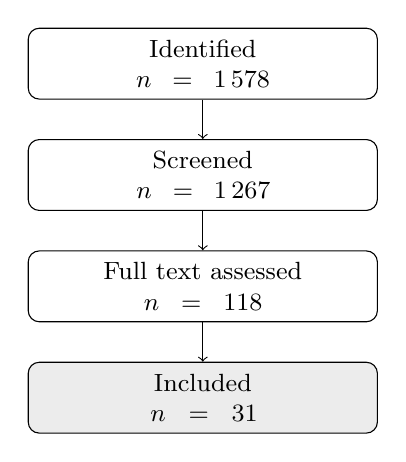
\begin{tikzpicture}[box/.style={draw,rounded corners,align=center,text width=4.2cm,minimum height=0.9cm,font=\small}, node distance=0.5cm]
  \node[box] (id) {Identified\\ $n = 1\,578$};
  \node[box,below=of id] (sc) {Screened\\ $n = 1\,267$};
  \node[box,below=of sc] (el) {Full text assessed\\ $n = 118$};
  \node[box,below=of el,fill=gray!15] (in) {Included\\ $n = 31$};
  \draw[->] (id) to (sc);
  \draw[->] (sc) to (el);
  \draw[->] (el) to (in);
\end{tikzpicture}
\caption{Simplified flow diagram. Keep the numbers in sync with Table~\ref{tab:prisma}.}
\end{figure}

\subsection{Study characteristics}
Summarise settings, sample sizes and interventions.

\subsection{Synthesis of results}
Report effect estimates with confidence intervals, or a structured narrative synthesis.

\section{Discussion}
Discuss the certainty of the evidence, limitations of the included studies and of the review process, and implications for practice and research.

\section{Other information}
\textbf{Registration:} give the registry and number. \textbf{Funding:} name sources. \textbf{Competing interests:} declare any.

\begin{thebibliography}{9}
\bibitem{page2021} M.~Example and co-authors, Reporting guideline for systematic reviews, \emph{Example Medical Journal} 372 (2021) 71--80.
\bibitem{trial1} A.~Researcher, Text message reminders in hypertension care: a randomised trial, \emph{Journal of Sample Trials} 8 (2019) 210--219.
\end{thebibliography}

\end{document}
